\documentclass[12pt,]{book}
\usepackage{lmodern}
\usepackage{amssymb,amsmath}
\usepackage{ifxetex,ifluatex}
\usepackage{fixltx2e} % provides \textsubscript
\ifnum 0\ifxetex 1\fi\ifluatex 1\fi=0 % if pdftex
  \usepackage[T1]{fontenc}
  \usepackage[utf8]{inputenc}
\else % if luatex or xelatex
  \ifxetex
    \usepackage{mathspec}
  \else
    \usepackage{fontspec}
  \fi
  \defaultfontfeatures{Ligatures=TeX,Scale=MatchLowercase}
\fi
% use upquote if available, for straight quotes in verbatim environments
\IfFileExists{upquote.sty}{\usepackage{upquote}}{}
% use microtype if available
\IfFileExists{microtype.sty}{%
\usepackage{microtype}
\UseMicrotypeSet[protrusion]{basicmath} % disable protrusion for tt fonts
}{}
\usepackage[margin=1in]{geometry}
\usepackage{hyperref}
\PassOptionsToPackage{usenames,dvipsnames}{color} % color is loaded by hyperref
\hypersetup{unicode=true,
            pdftitle={AllCCS Tutorial V1.00},
            pdfauthor={Zhiwei Zhou},
            colorlinks=true,
            linkcolor=Maroon,
            citecolor=Blue,
            urlcolor=Blue,
            breaklinks=true}
\urlstyle{same}  % don't use monospace font for urls
\usepackage{natbib}
\bibliographystyle{apalike}
\usepackage{longtable,booktabs}
\usepackage{graphicx,grffile}
\makeatletter
\def\maxwidth{\ifdim\Gin@nat@width>\linewidth\linewidth\else\Gin@nat@width\fi}
\def\maxheight{\ifdim\Gin@nat@height>\textheight\textheight\else\Gin@nat@height\fi}
\makeatother
% Scale images if necessary, so that they will not overflow the page
% margins by default, and it is still possible to overwrite the defaults
% using explicit options in \includegraphics[width, height, ...]{}
\setkeys{Gin}{width=\maxwidth,height=\maxheight,keepaspectratio}
\IfFileExists{parskip.sty}{%
\usepackage{parskip}
}{% else
\setlength{\parindent}{0pt}
\setlength{\parskip}{6pt plus 2pt minus 1pt}
}
\setlength{\emergencystretch}{3em}  % prevent overfull lines
\providecommand{\tightlist}{%
  \setlength{\itemsep}{0pt}\setlength{\parskip}{0pt}}
\setcounter{secnumdepth}{5}
% Redefines (sub)paragraphs to behave more like sections
\ifx\paragraph\undefined\else
\let\oldparagraph\paragraph
\renewcommand{\paragraph}[1]{\oldparagraph{#1}\mbox{}}
\fi
\ifx\subparagraph\undefined\else
\let\oldsubparagraph\subparagraph
\renewcommand{\subparagraph}[1]{\oldsubparagraph{#1}\mbox{}}
\fi

%%% Use protect on footnotes to avoid problems with footnotes in titles
\let\rmarkdownfootnote\footnote%
\def\footnote{\protect\rmarkdownfootnote}

%%% Change title format to be more compact
\usepackage{titling}

% Create subtitle command for use in maketitle
\newcommand{\subtitle}[1]{
  \posttitle{
    \begin{center}\large#1\end{center}
    }
}

\setlength{\droptitle}{-2em}

  \title{AllCCS Tutorial V1.00}
    \pretitle{\vspace{\droptitle}\centering\huge}
  \posttitle{\par}
    \author{Zhiwei Zhou}
    \preauthor{\centering\large\emph}
  \postauthor{\par}
      \predate{\centering\large\emph}
  \postdate{\par}
    \date{2019-11-01}

\usepackage{booktabs}

\begin{document}
\maketitle

{
\hypersetup{linkcolor=black}
\setcounter{tocdepth}{1}
\tableofcontents
}
\listoftables
\listoffigures
\chapter*{About AllCCS}\label{about-allccs}
\addcontentsline{toc}{chapter}{About AllCCS}

Copyright (c) 2019 AllCCS Development Team

\href{http://allccs.zhulab.cn/}{\textbf{AllCCS}} is a powerful platform
to support various applications in Ion Mobility -- Mass Spectrometry
(IM-MS). It is designed to contain three major parts: \textbf{1) Unified
CCS database, 2) Machine learning based CCS prediction, and 3) small
molecule annotation}. The unified CCS database is one of the most
comprehensive CCS databases, covering \textasciitilde{}1,700,000 small
molecules. It provides a universal platform to contain both experimental
CCS values (3,539) and predicted CCS values (over 10,000,000). Machine
learning based CCS prediction function supports convenient prediction
from SMILES structure to CCS values. This function utilizes the second
generation CCS prediction algorithm to generate CCS values and RSS score
for novel structures. Small molecule annotation provides an easy-to-use
annotation function for various features or compounds. It is supported
to search database with measured m/z and CCS for annotation, or in
conjunct with any other annotation tools, such as MetFrag, CFM-ID,
MS-Finder, and SIRUS etc.

Zhiwei Zhou (\url{zhouzw@sioc.ac.cn}) Zheng-Jiang Zhu
(\url{jiangzhu@sioc.ac.cn}) \href{http://www.zhulab.cn/}{Laboratory for
Mass Spectrometry and Metabolomics}
\href{http://www.ircbc.ac.cn/}{IRCBC}, Shanghai Institute of Organic
Chemistry Chinese Academy of Sciences, Shanghai, China

\chapter*{Citation}\label{citation}
\addcontentsline{toc}{chapter}{Citation}

If AllCCS is useful in your project, please cite our articles.

\begin{itemize}
\tightlist
\item
  Z. Zhou, Z.-J. Zhu* etc. Advancing CCS database towards metabolite
  annotation, In preparing
\end{itemize}

\chapter*{News}\label{news}
\addcontentsline{toc}{chapter}{News}

\textbf{November 6, 2019}

\begin{itemize}
\tightlist
\item
  Test in web server
\item
  Fix bugs in admin system
\item
  Fix some known bugs
\item
  Update formal database and install AllCCS package V0.1.61
\item
  Correct compound name of drugbank compound 
\end{itemize}

\textbf{September 22, 2019}

\begin{itemize}
\tightlist
\item
  Demo webserver online
\end{itemize}

\chapter{Quick Start Guide}\label{quick-start-guide}

\section{Create a AllCCS Account}\label{create-a-allccs-account}

Users need to register AllCCS account to use the webserver. This process
is very sample, and \textbf{completely private}. To register an account,
navigate to the home page. The ``Sign up'' button is in the upper right
corner of the page. Then, you need to fill in your email and
verification code which would be sent to your email (Figure
\ref{fig:FigRegister}). Finally, input some basic information to
complete the registration. You could log in and enjoy all functions in
the web server.

\begin{figure}

{\centering 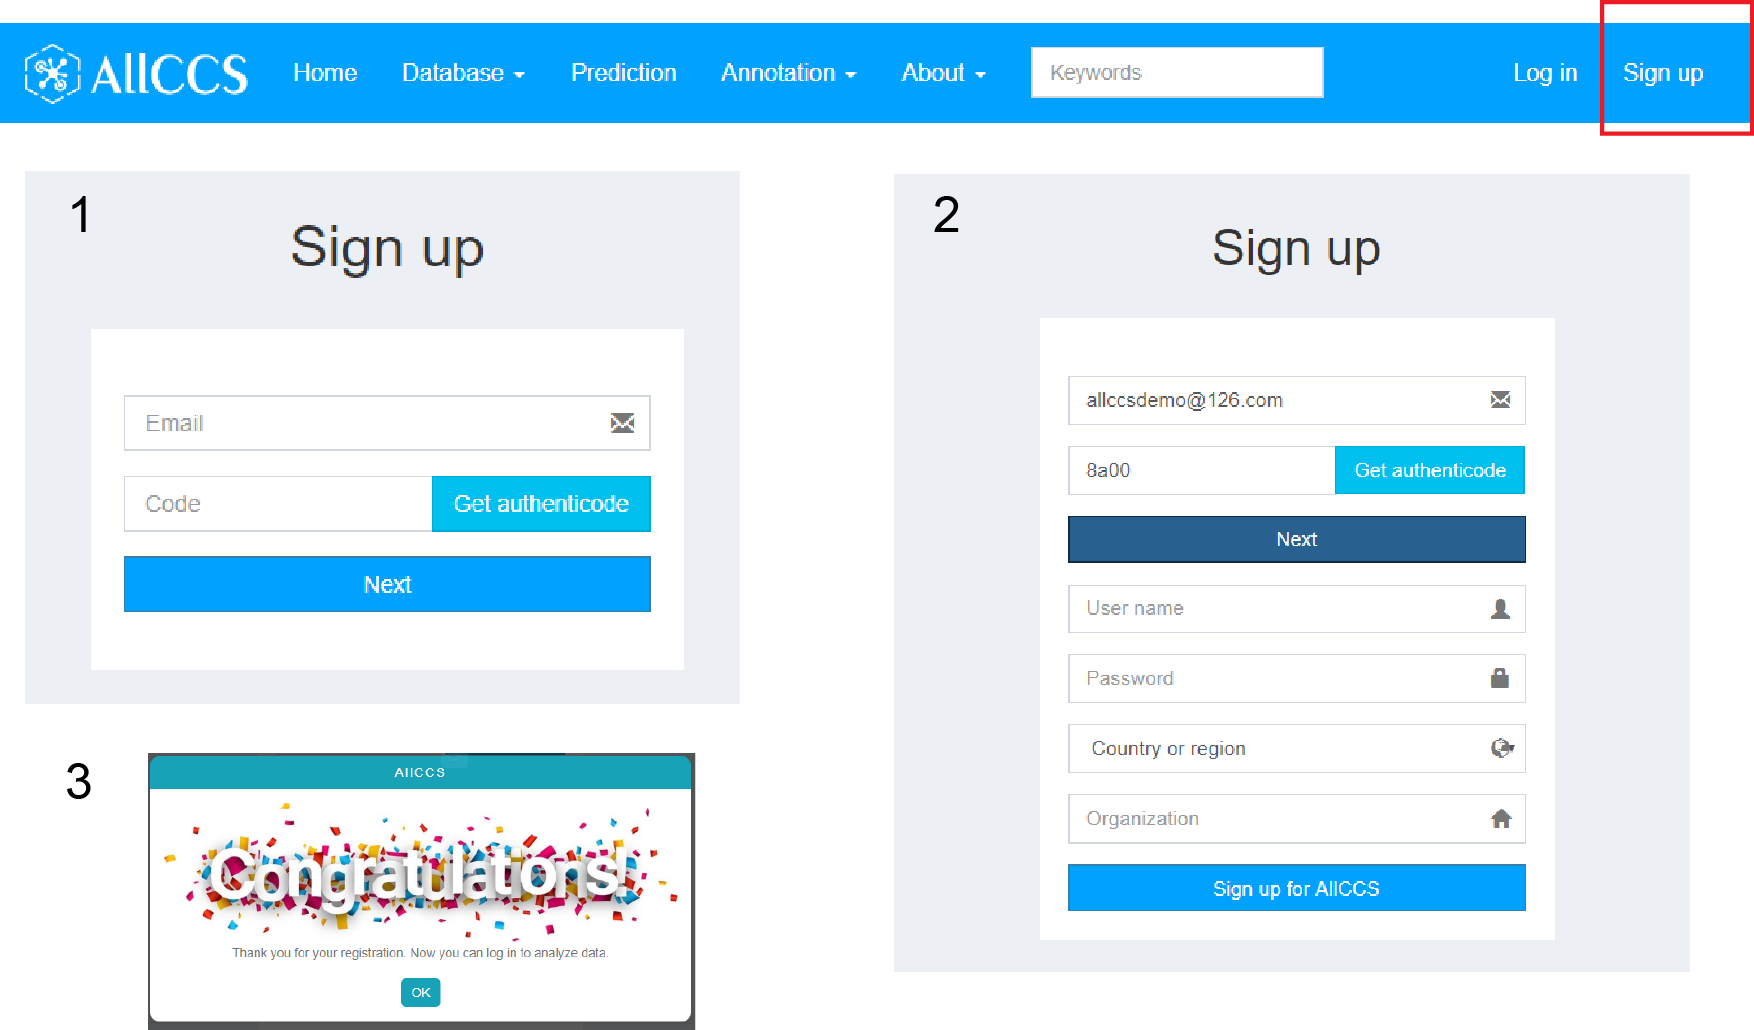
\includegraphics{images/chapter1/register_1} 

}

\caption{Register AllCCS account}\label{fig:FigRegister}
\end{figure}

\section{Browser CCS database}\label{browser-ccs-database}

You could search you interested compound (name, formula, smiles, inchi,
InChIKey etc.) in the search box in navigation bar, or directly browser
the all database records in the ``browser'' page (Figure
\ref{fig:FigBrowser1}).

\begin{figure}

{\centering 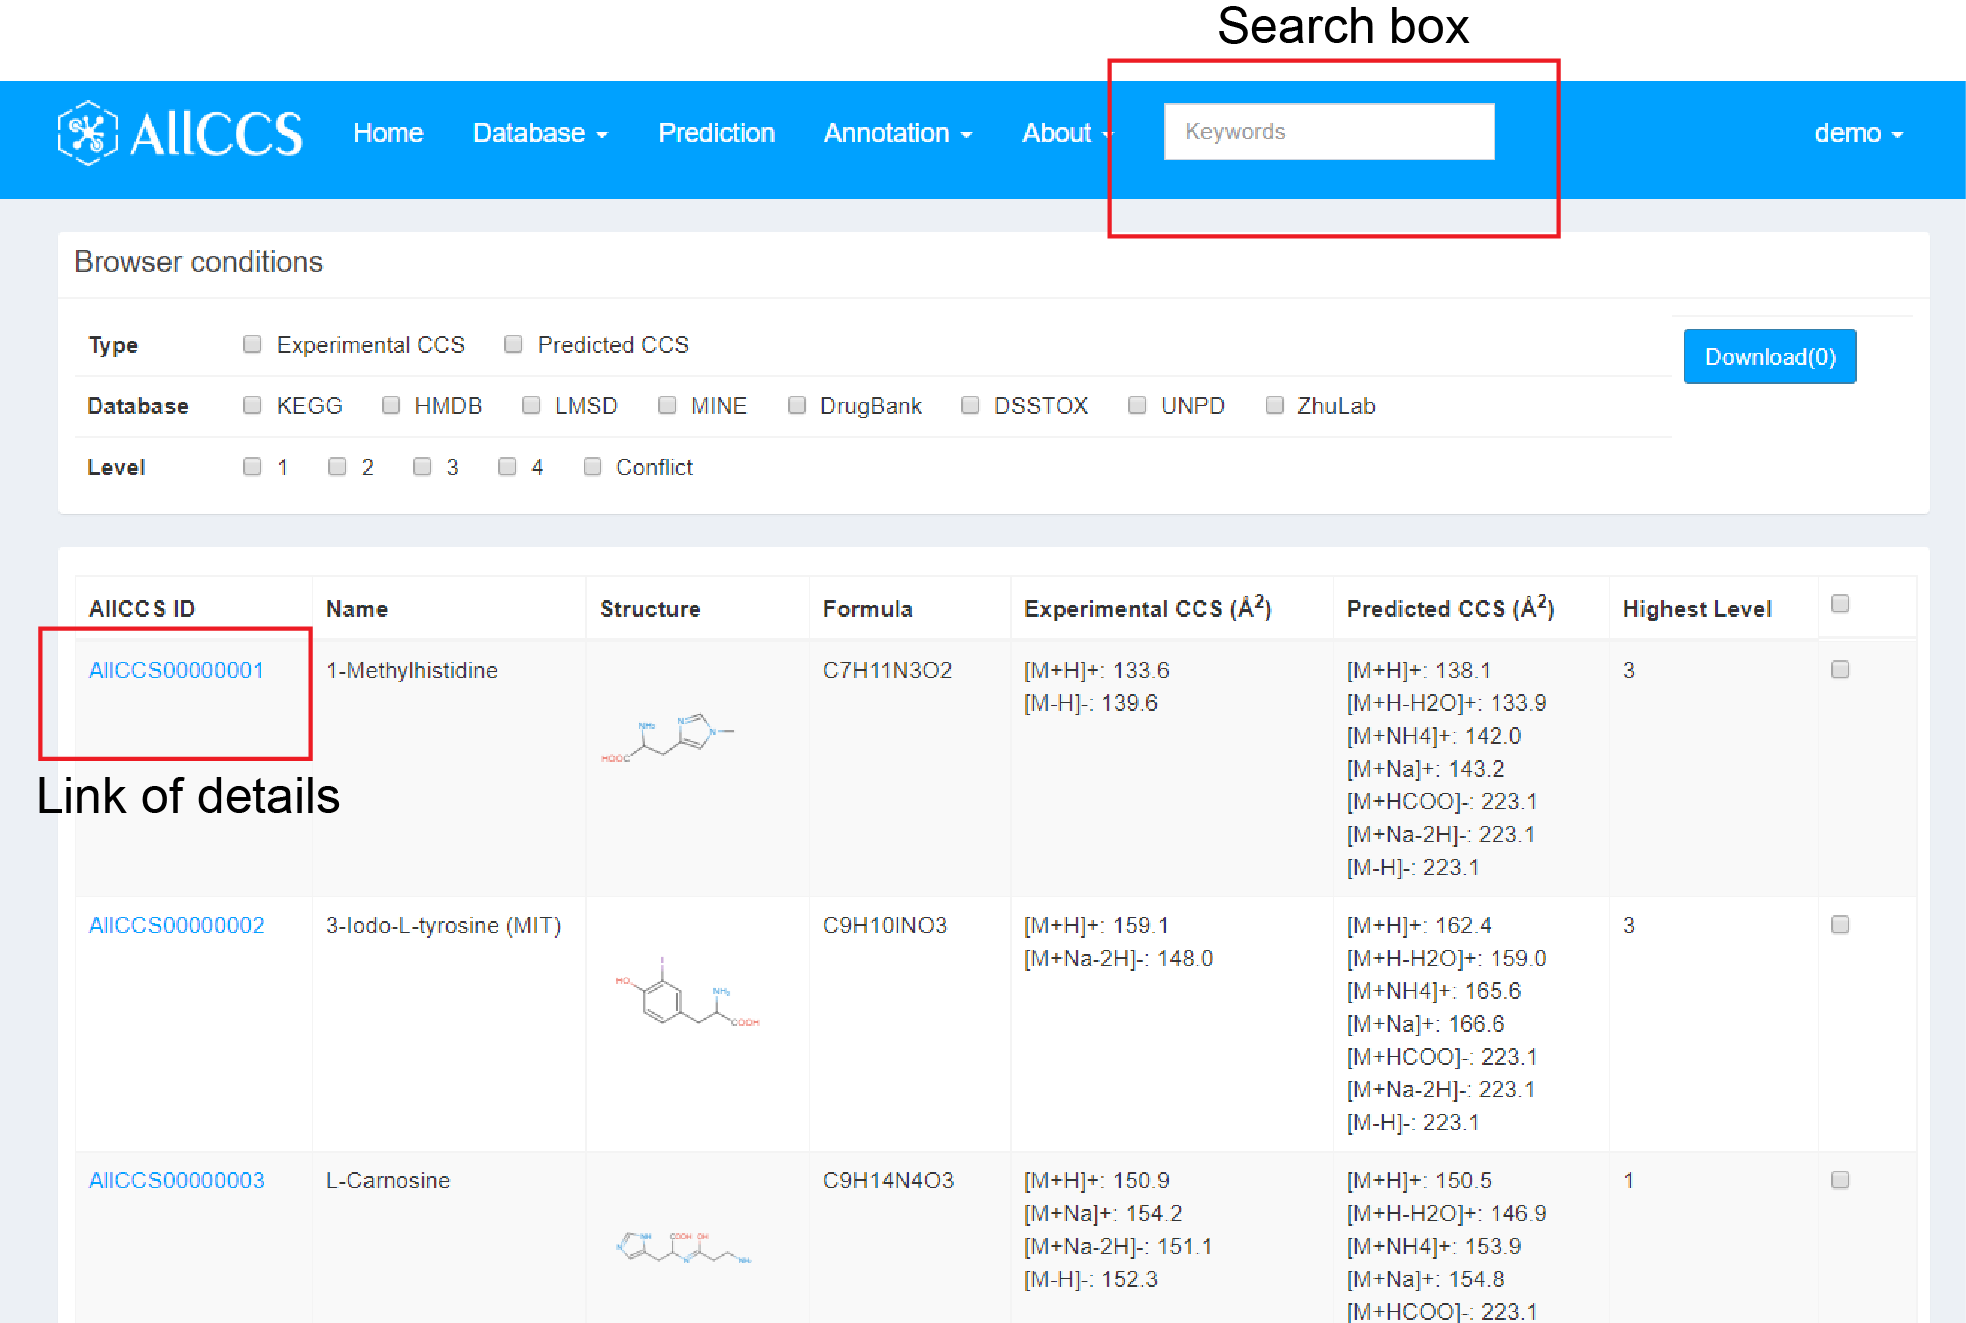
\includegraphics{images/chapter1/browser_1} 

}

\caption{Register AllCCS account}\label{fig:FigBrowser1}
\end{figure}

Then, you can click the link in the column of AllCCS ID to browser
detail information of this compound (Figure \ref{fig:FigBrowser2}). It
includes basic meta information, unified CCS values, experimental CCS
records, predicted CCS records and other database links etc. Please see
section \ref{ccsdb} for more details.

\begin{figure}

{\centering 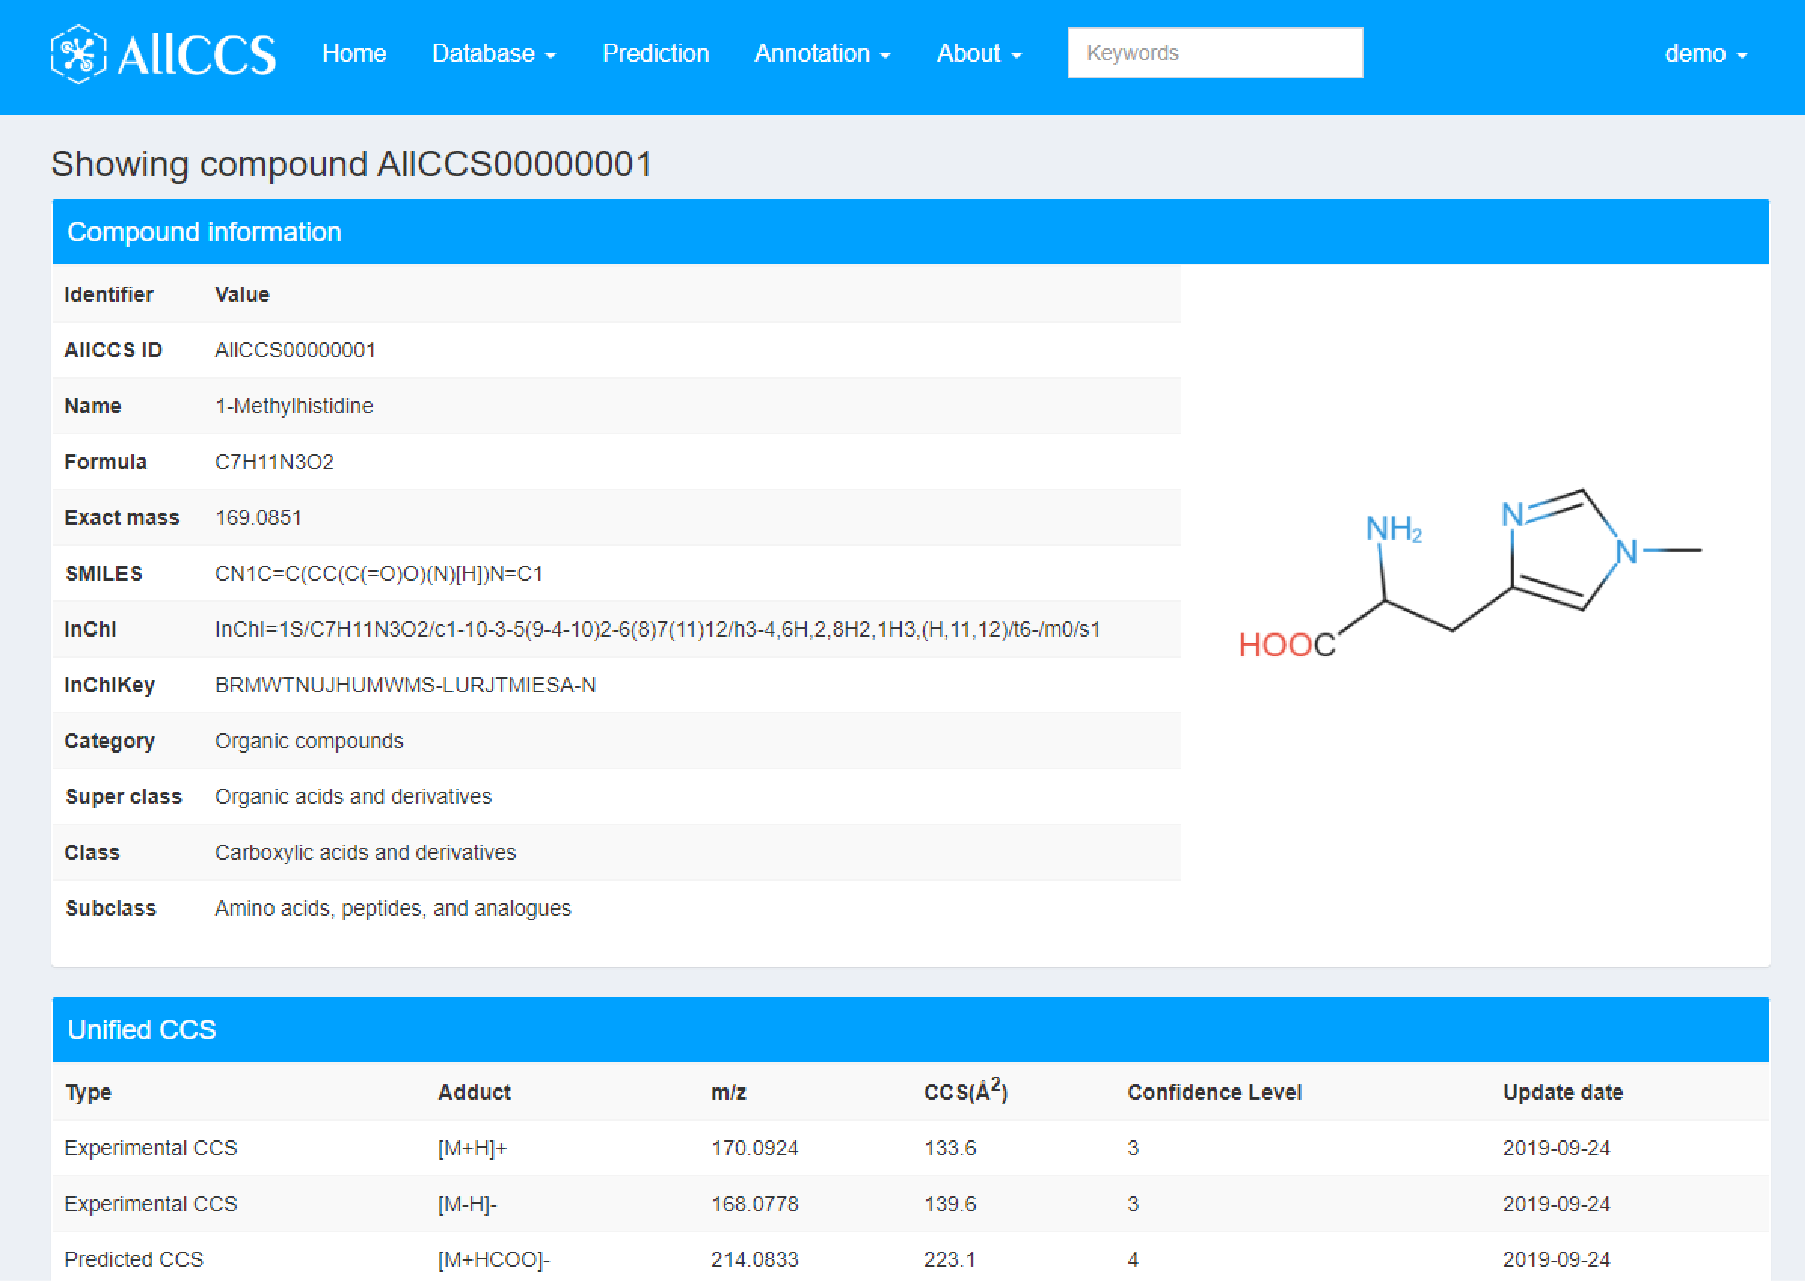
\includegraphics{images/chapter1/browser_2} 

}

\caption{Register AllCCS account}\label{fig:FigBrowser2}
\end{figure}

\section{Perform CCS
prediction/Annotation}\label{perform-ccs-predictionannotation}

AllCCS also provides CCS prediction function (Section
\ref{ccsprediction}) and metabolite annotation functions (Section
\ref{metannotation}). You could click the link or corresponding item in
navigation bar. For CCS prediction function, please input the SMILES
list of your compounds in the input panel. The result would be returned
on the project panel within several seconds (Figure
\ref{fig:FigPrediction}).

\begin{figure}

{\centering 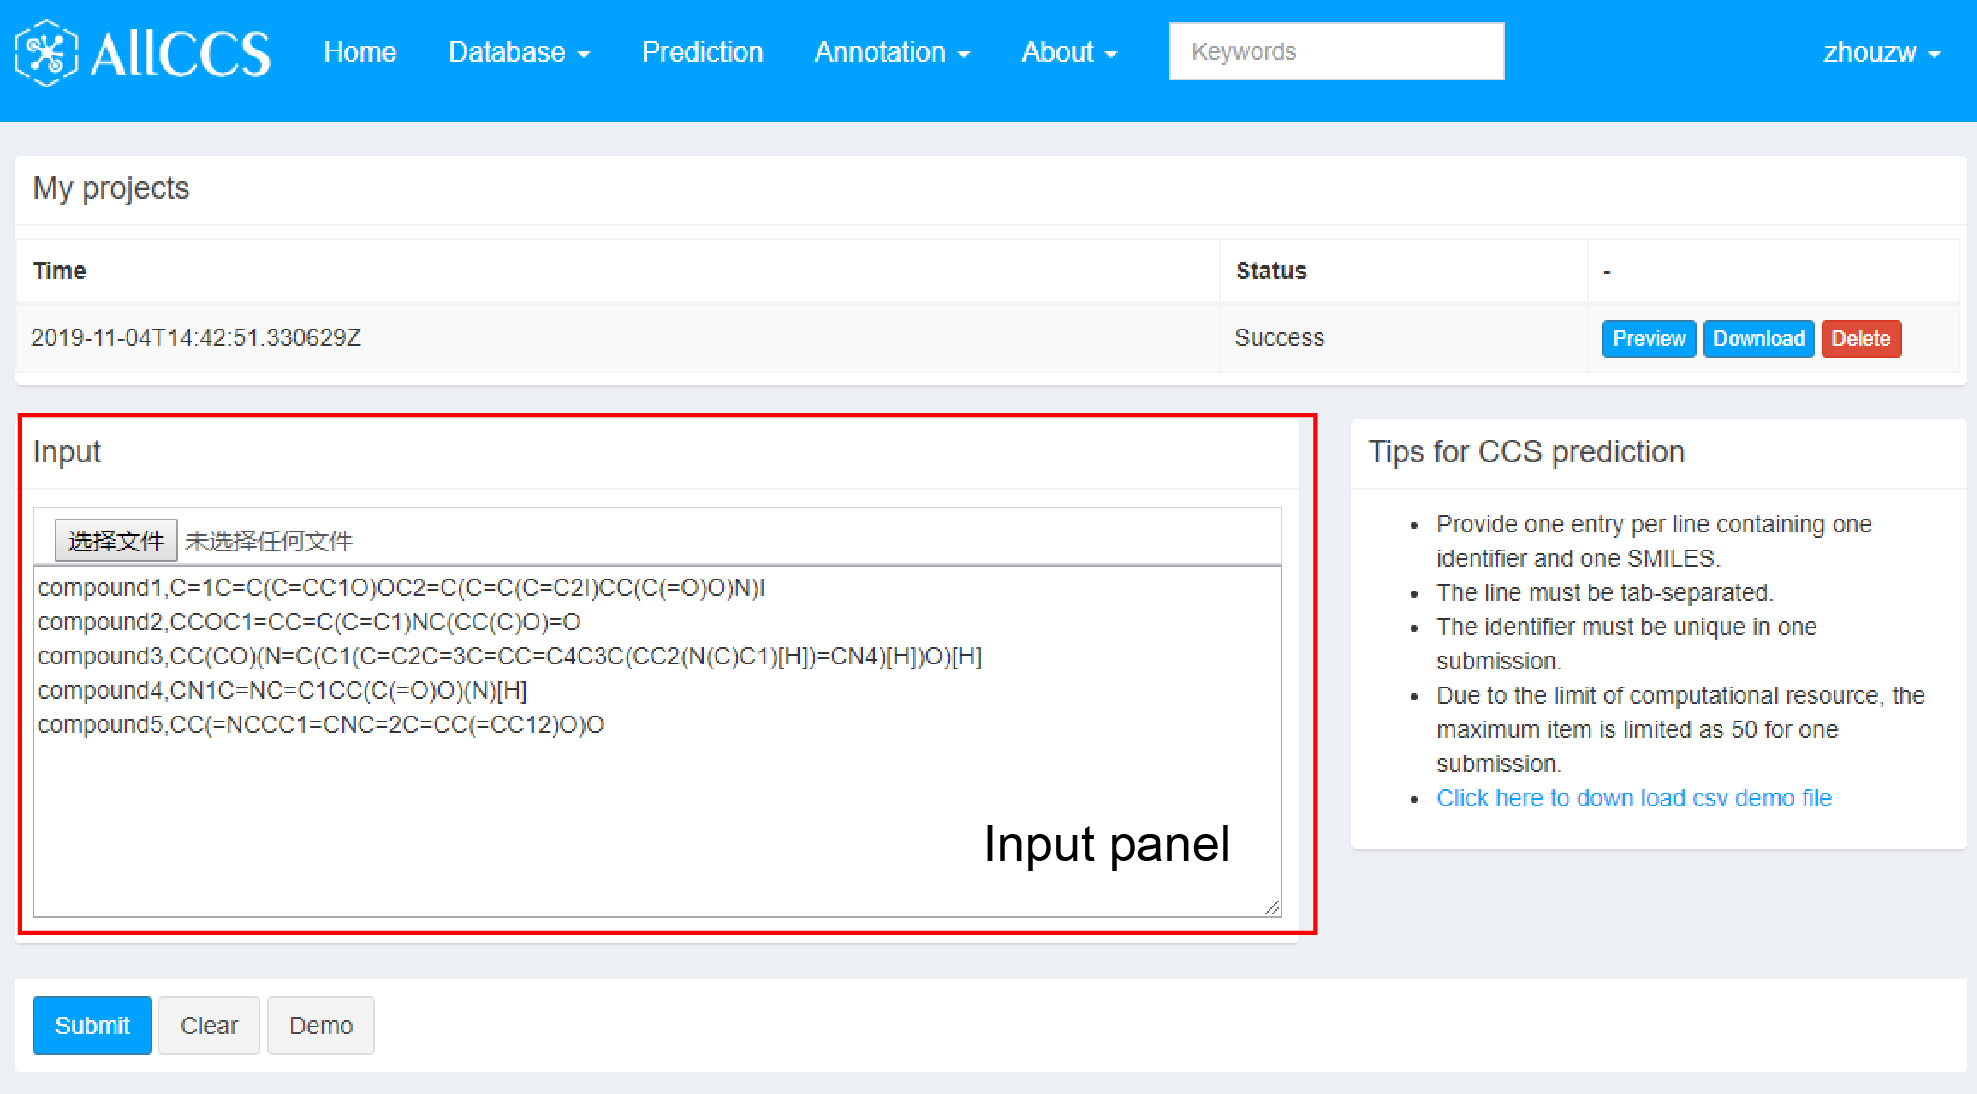
\includegraphics{images/chapter1/prediction} 

}

\caption{Register AllCCS account}\label{fig:FigPrediction}
\end{figure}

For annotation function, you could search experimental feature to search
the database with your settings, or filter/rerank candidates to conjunct
with MS/MS annotation tools (Figure \ref{fig:FigMatch}).

\begin{figure}

{\centering 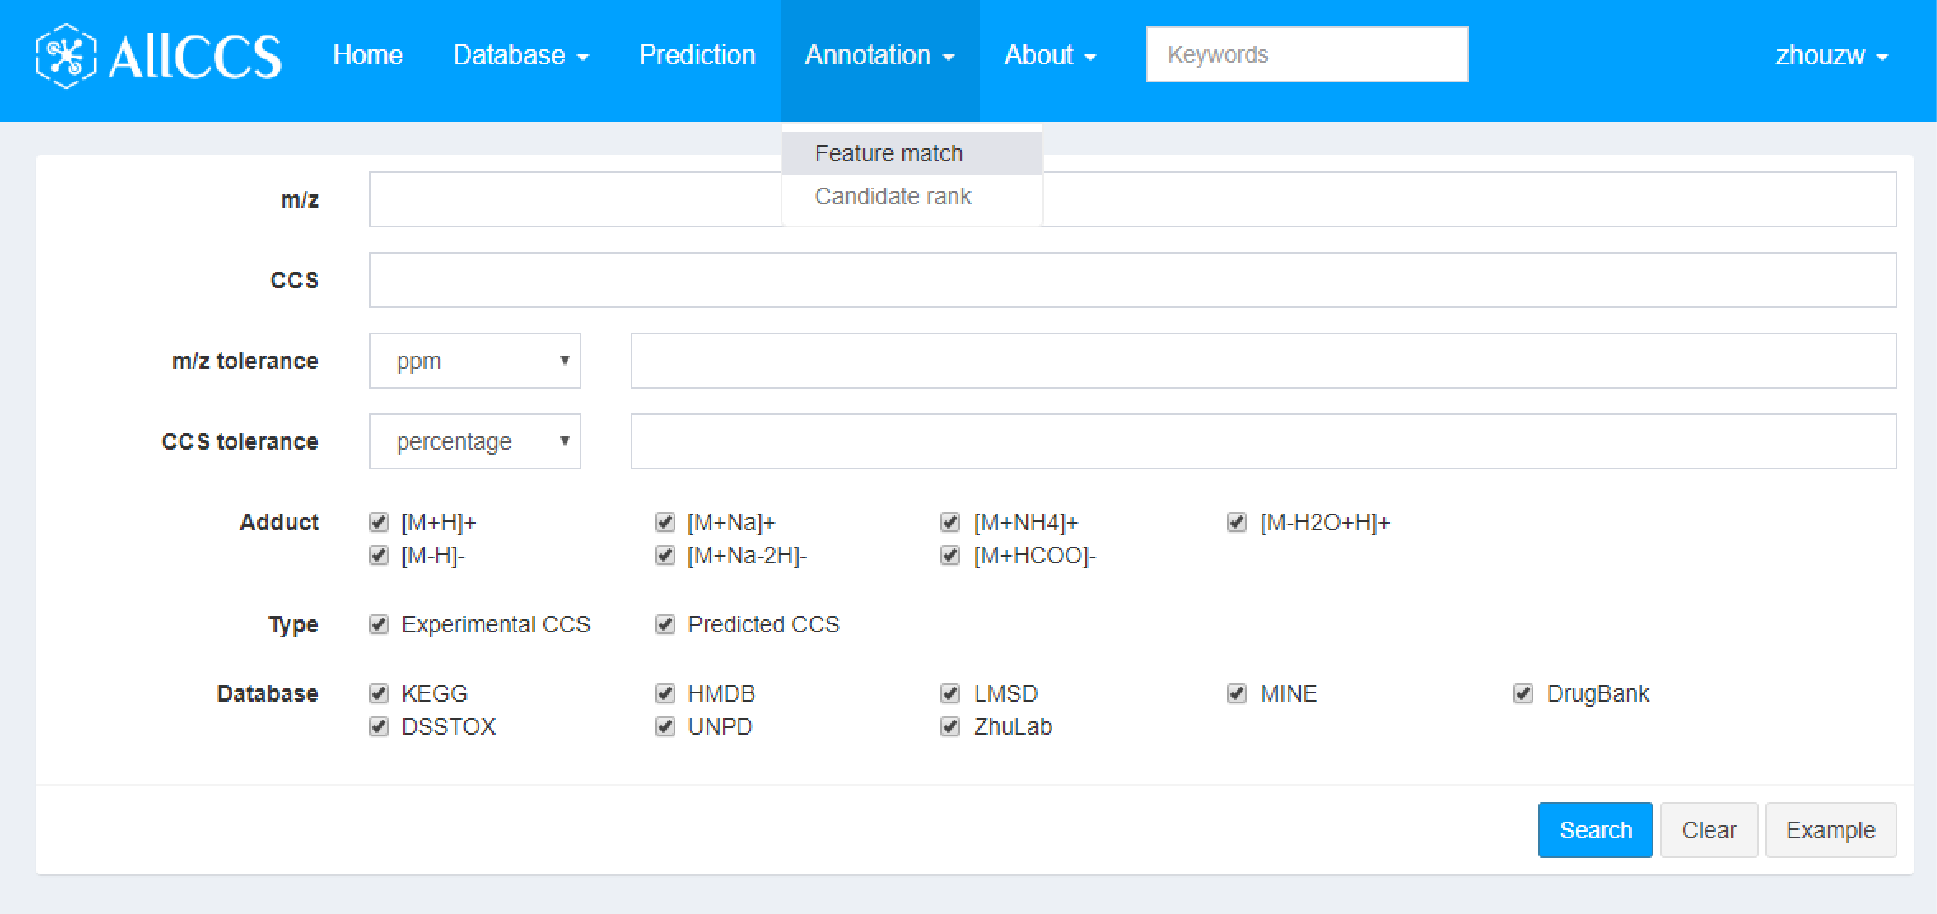
\includegraphics{images/chapter1/match} 

}

\caption{Register AllCCS account}\label{fig:FigMatch}
\end{figure}

\chapter{CCS Database}\label{ccsdb}

\section{Compound Browser}\label{compound-browser}

\section{Compound Card}\label{compound-card}

\section{Advanced Search}\label{advanced-search}

\chapter{CCS Prediction}\label{ccsprediction}

\chapter{Metabolite Annotation}\label{metannotation}

We have finished a nice book.

\bibliography{book.bib,packages.bib}


\end{document}
